\documentclass{VRARWorkshop}

\usepackage[utf8]{inputenc}
\usepackage[T1]{fontenc}
\usepackage[hidelinks]{hyperref}

\title{Augmented reality for supporting manual non-destructive ultrasonic testing of metal pipes and plates}

%\authors{Robert Deppe, Oliver Nemitz, Jens Herder}
\authors{~}

\affiliations{~}
% TODO: Correct affiliations

\abstract{
We describe an application of augmented reality technology for non-destructive testing of products in the metal-industry.
The prototype is created with hard- and software, that is usually employed in the gaming industry, and delivers positions for creating ultrasonic material scans (c-scans).
Using a stereo camera in combination with an {\sc hmd} enables realtime visualisation of the probes path, as well as the setting of virtual markers on the specimen.
As a part of the implementation the downhill simplex optimization algorithm is implemented to fit the specimen to a cloud of recorded surface points.
The accuracy is statistically tested and evaluated with the result, that the tracking system is accurate up to ca. 1-2 millimeters in well set-up conditions.
This paper is of interest not only for research institutes of the metal-industry, but also for any areas of work, in which the enhancement with augmented reality is possible and a price tracking is necessary.
}

% Give some keywords
\keywords{
Nondestructive Testing,
Ultrasonic,
Augmented Reality,
Tracking,
Stereo camera,
head mounted display,
NDT,
AR
}

\begin{document}

\section{Introduction}

In the field of nondestructive testing of steel products, the ultrasonic (US) inspection is a frequently used method to assure given safety requirements. For heavy plates and large diameter pipes the manual US testing is often applied as a follow-up inspection. Here, a US probe is moved by hand on the surface of the specimen (cf. Figure \ref{fig:manual_UT}). While moving and possibly rotating the probe the operator monitors the US signal on a screen. Usually, in case of an imperfection in the material, the US signal exhibits a higher amplitude and the position of the imperfection can be marked on the specimen.
However, the exact position and orientation of the probe are not captured during the manual inspection. Hence, generating an objective report with for example a map of color coded US amplitudes onto probe positions (C-Scan) is not directly possible. Furthermore, there is usually no kind of tracking and visualization of those parts of the specimen surface which have already been inspected and especially no control if inspection gaps occur.
The aim of our system is therefore to track the position and orientation of the US probe during the inspection and assign them to the corresponding US signals. This tracking is done with standard AR/VR components of an HTC Vive system. Global coordinates of the probe are converted to coordinates in a local coordinate system on the specimen and sent to a UT inspection software which can generate a C-Scan of the inspection. By a ZED mini stereo camera it is possible to view the inspection in AR and to visualize certain virtual elements as the pathes of the already inspected areas.

\begin{figure}[h!]
    \begin{center}
        \includegraphics[width=120mm]{images/US-workspace}
        \caption{\label{fig:manual_UT} Manual ultrasonic testing of steel large diameter pipes.}
    \end{center}
\end{figure}

\begin{figure}[h!]
    \begin{center}
        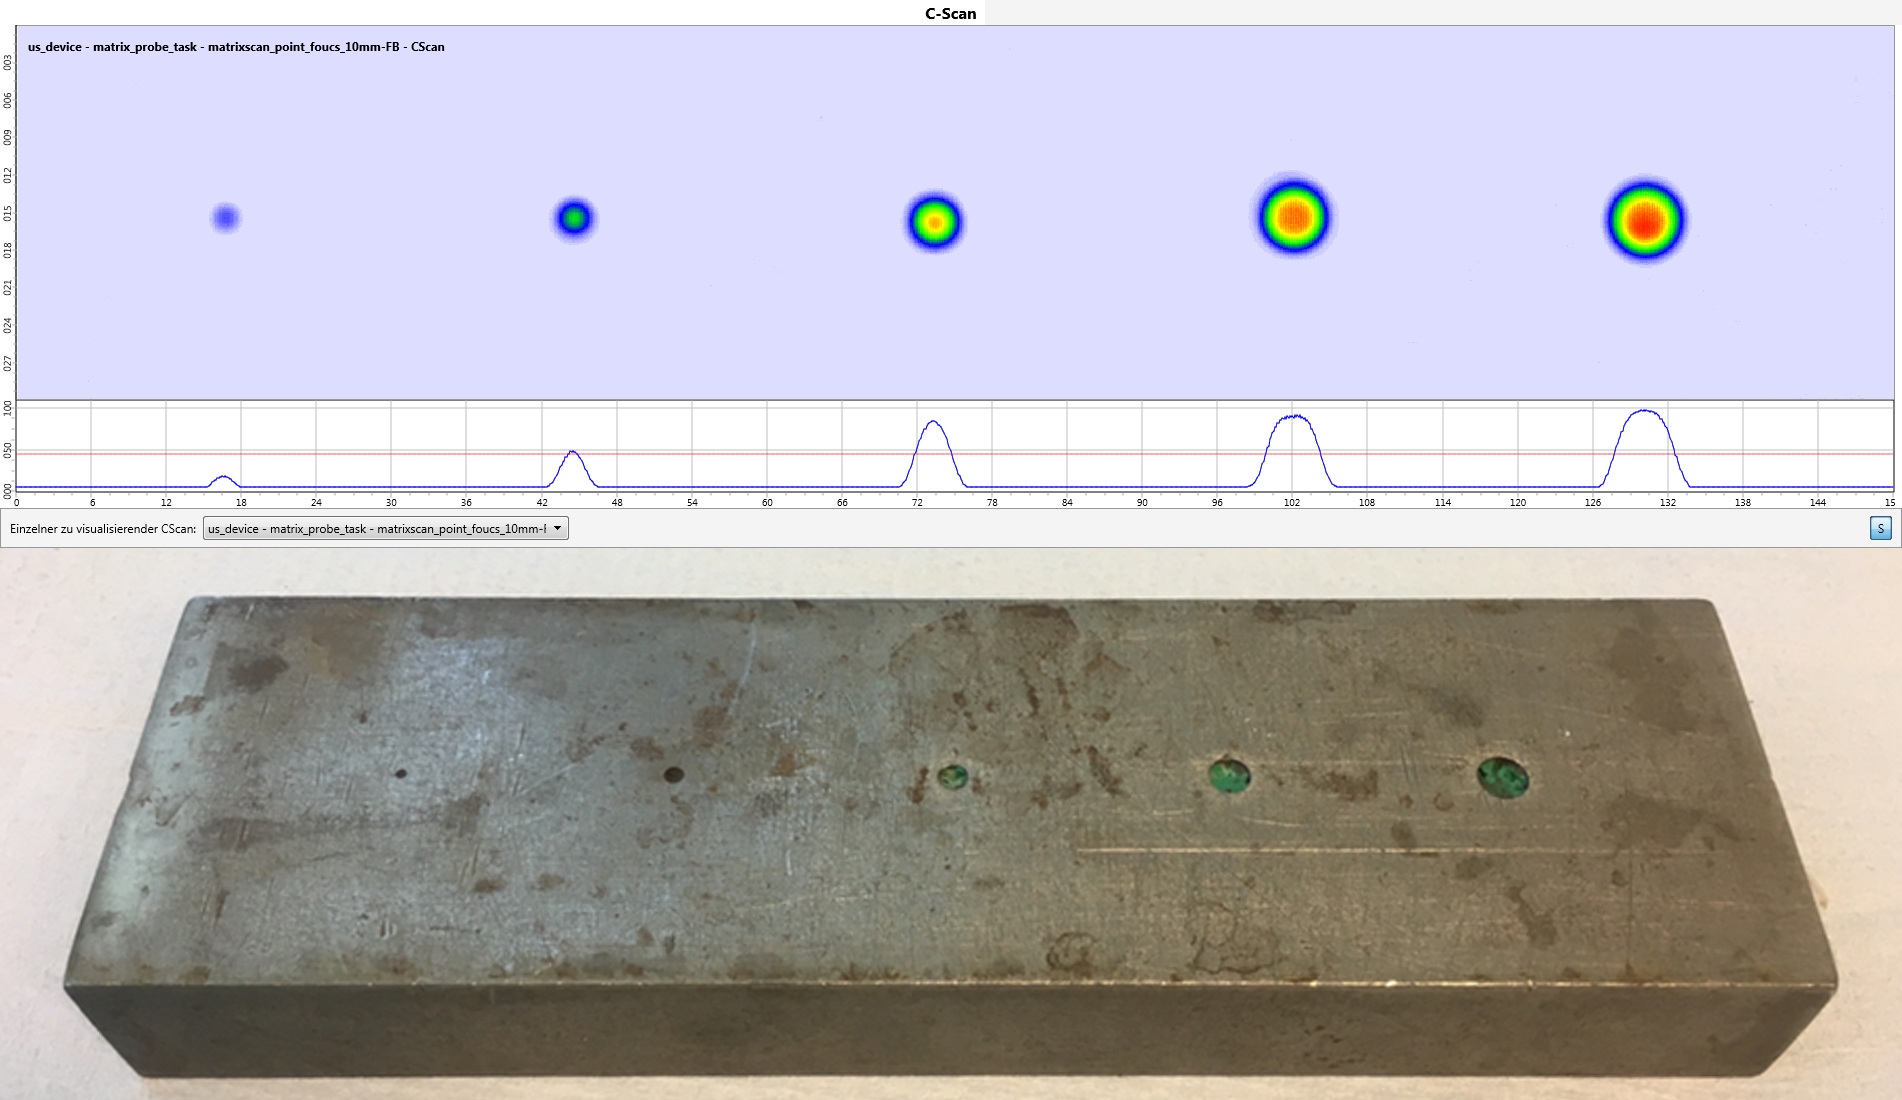
\includegraphics[width=90mm]{images/CScan}
        \caption{\label{fig:cScan} C-Scan with a resolution of 0,1\,mm}
    \end{center}
\end{figure}

\section{Related Research}
In the 2015 released patent \textit{A system and method of non-destructive inspection with a visual scanning guide} \textit{Olympus} patented the procedure of enhancing the manual inspection with AR-Glasses which help to trace a predefined inspection-plan path.
The patent describes details like tolerated deviation from the inspection path.
However there is no mentioning of the possibility to log specific points or the traced path on the probe \cite{ARPat15}.\\

The article \textit{Non-contact tracking of phased-array probe and real-time generation of C-scans for the inspection of composite aerospace structures} describes a system, which uses a stereocamera and active markers to determine the probes position and orientation on a possibly curved surface of plane components \cite{walter_non-contact_2007}.\\

A similar system, supporting the cleaning of surfaces is presented in the article \textit{Cleaning Up With Augmented Reality} by Alice Bonasio.
It describes the advantages of using AR-technology, like a DRAW or HYBRID system (section~\ref{sec:DrawVsErase}), can have on quality assurance in the commercial cleaning industry \cite{ARClean}.\\

\cite{fadzil_design_2015}\\

\section{Basics of non-destructive ultrasonic testing of metal products}
\cite{deutsch_zfp_2010}
\cite{moles_introduction_2004}
\cite{olympus_Grundlagen}

\section{Description of the AR-application}
The AR-application supports manual testing visually, and sends the aquired position data to the inspection software, which is connected via an IP connection.
Through a AR-HMD the inspector is able to see the already inspected path and identify gaps.
Position and Rotation is send to the ultrasonic scanning computer, where the data is combined with the measurements received by the probe into a C-Scan.

\section{Implementation}
The application was implemented in the game-engine Unity.
Attached to the HMD is the \textit{ZEDmini}, a stereo-camera that can be used to display a camera image in the HMD and to create a depth mask.

\cite{dorner_virtual_2013}

\begin{figure}[h!]
    \begin{center}
        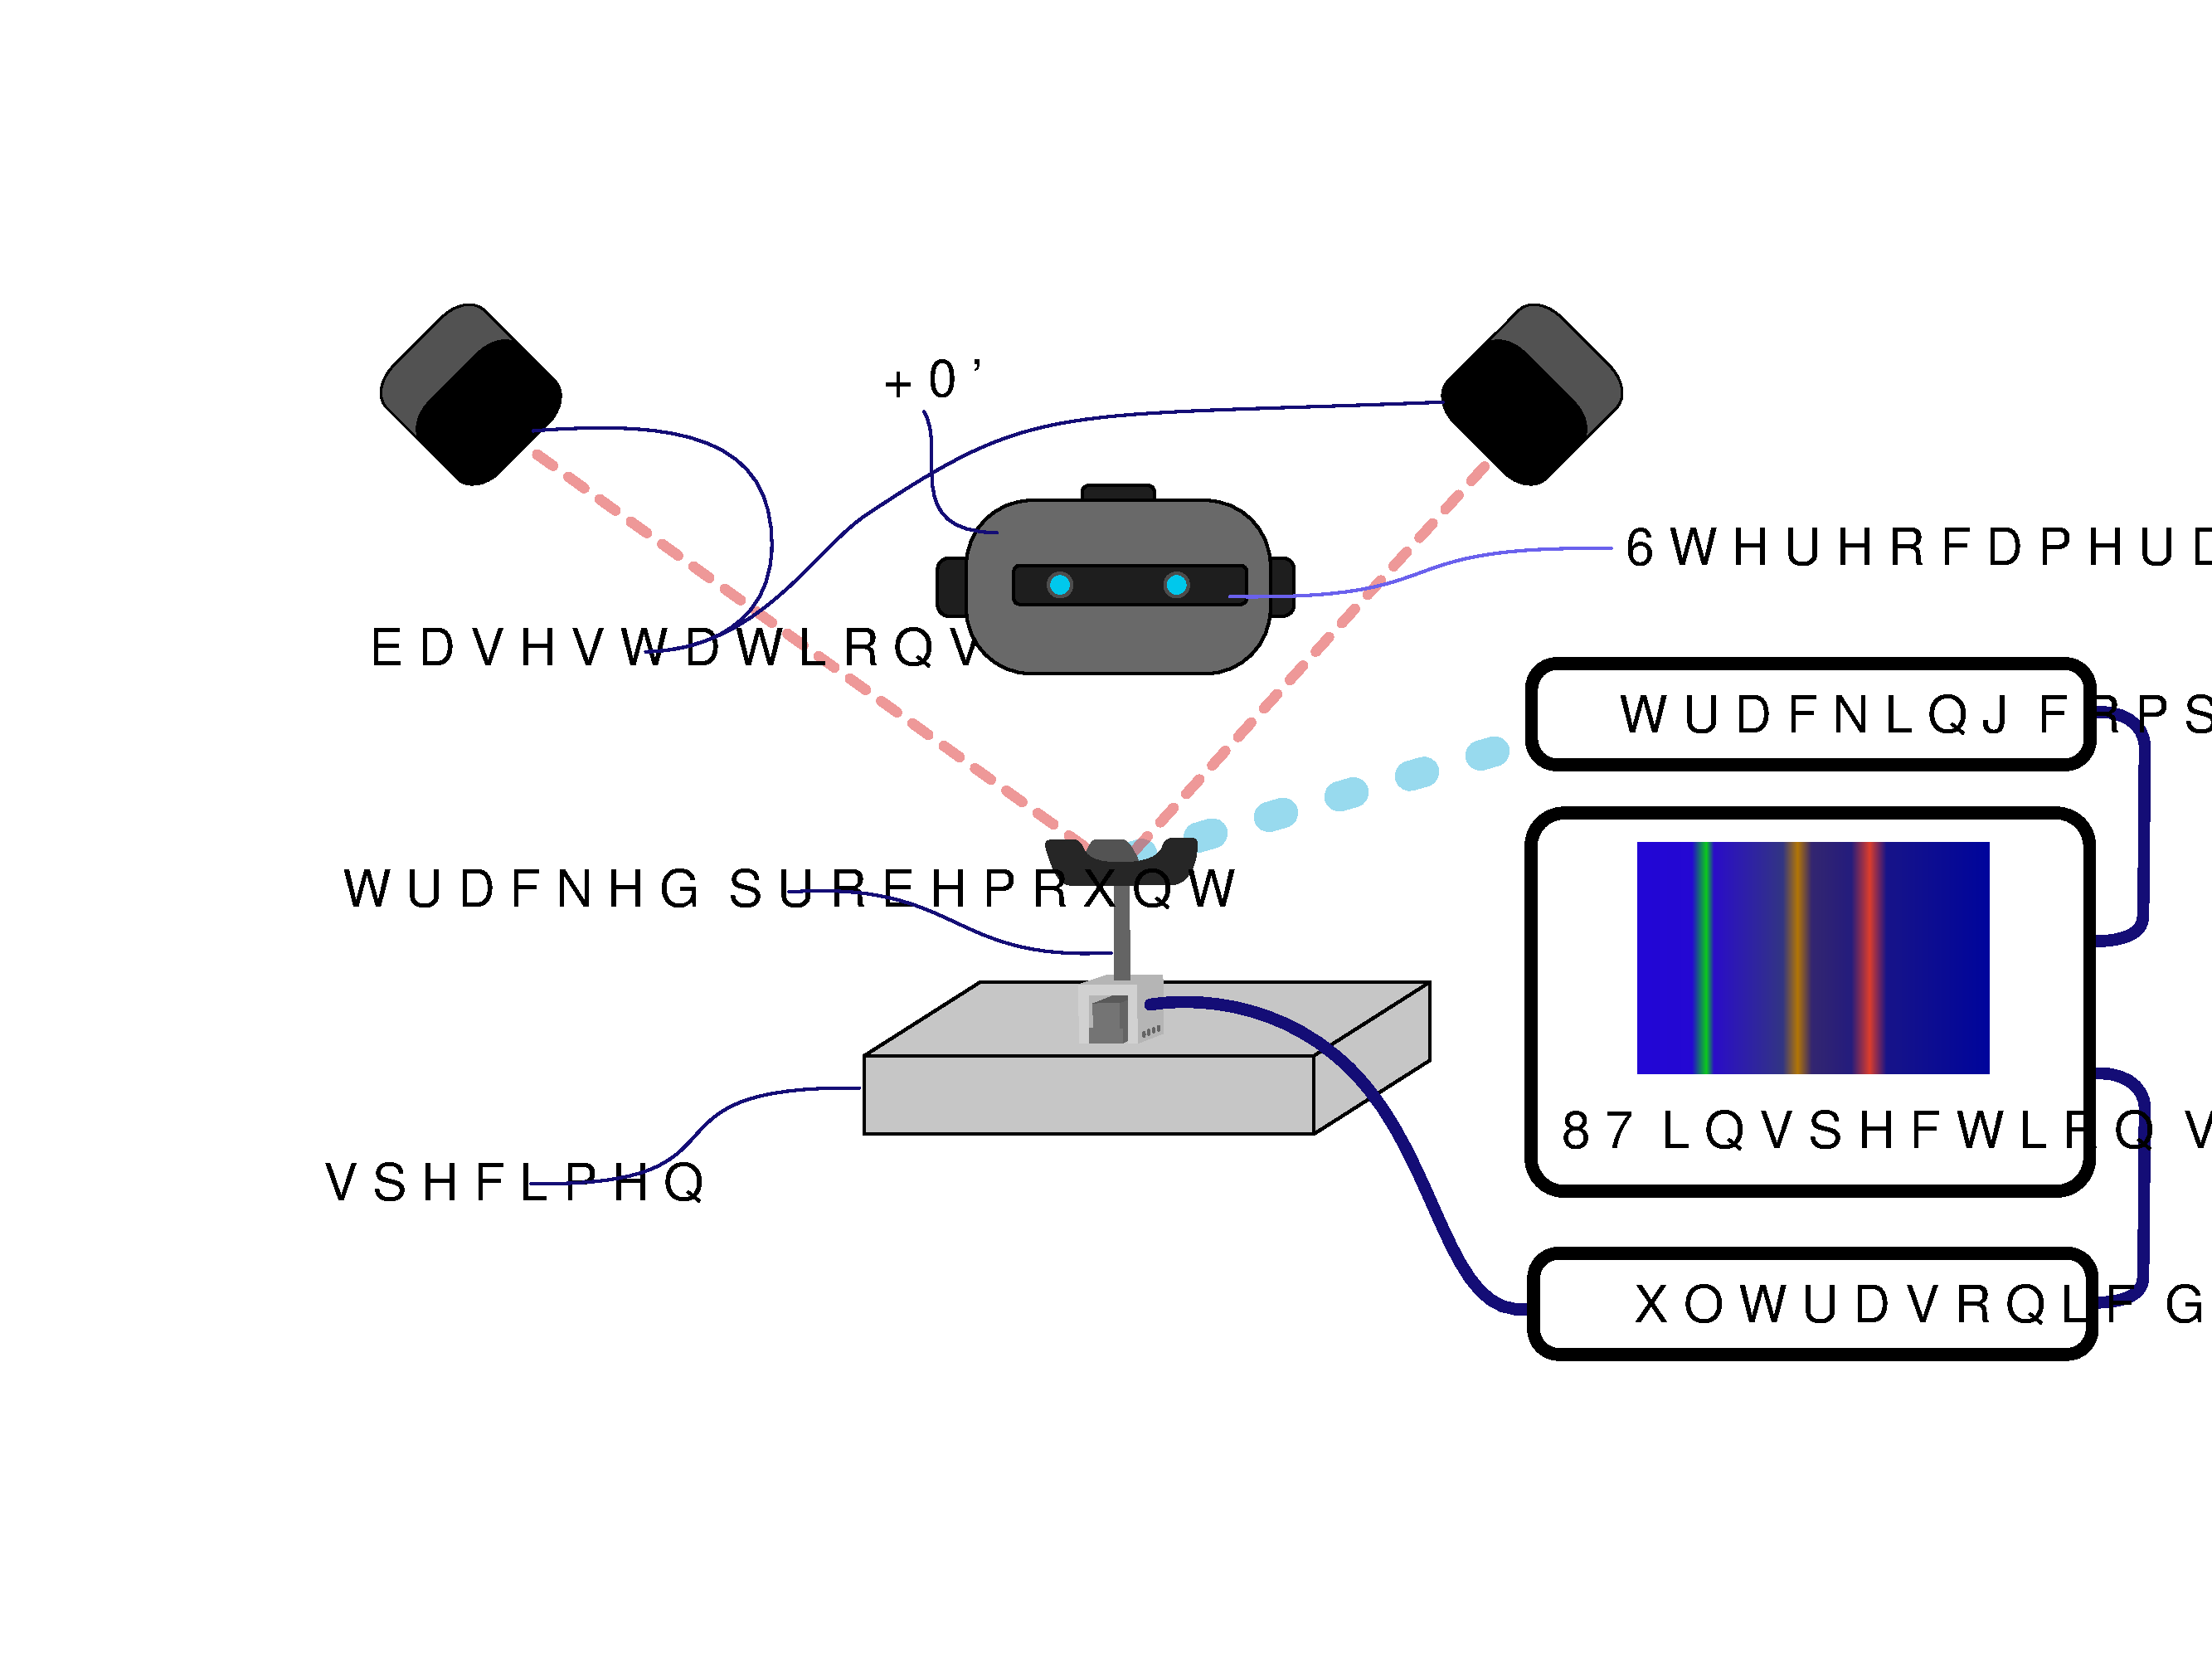
\includegraphics[width=158mm]{images/Setup-ARUS}
        \caption{\label{fig:Setup} Setup of the described AR-application.}
    \end{center}
\end{figure}

\subsection{Tracking of the ultrasonic probe}
The ultrasonic probe is tracked with the help of a attachable tracked \textit{VIVE}-Tracker.
This Tracker is attached to a mount, in which the ultrasonic probe is fixed (figure~\ref{fig:probemount}).
The offset and orientation between the tracker and probe is applied in software by setting the virtual probe as a child transform of the tracker.

\begin{figure}[h!]
  \label{fig:probemount}
    \begin{center}
        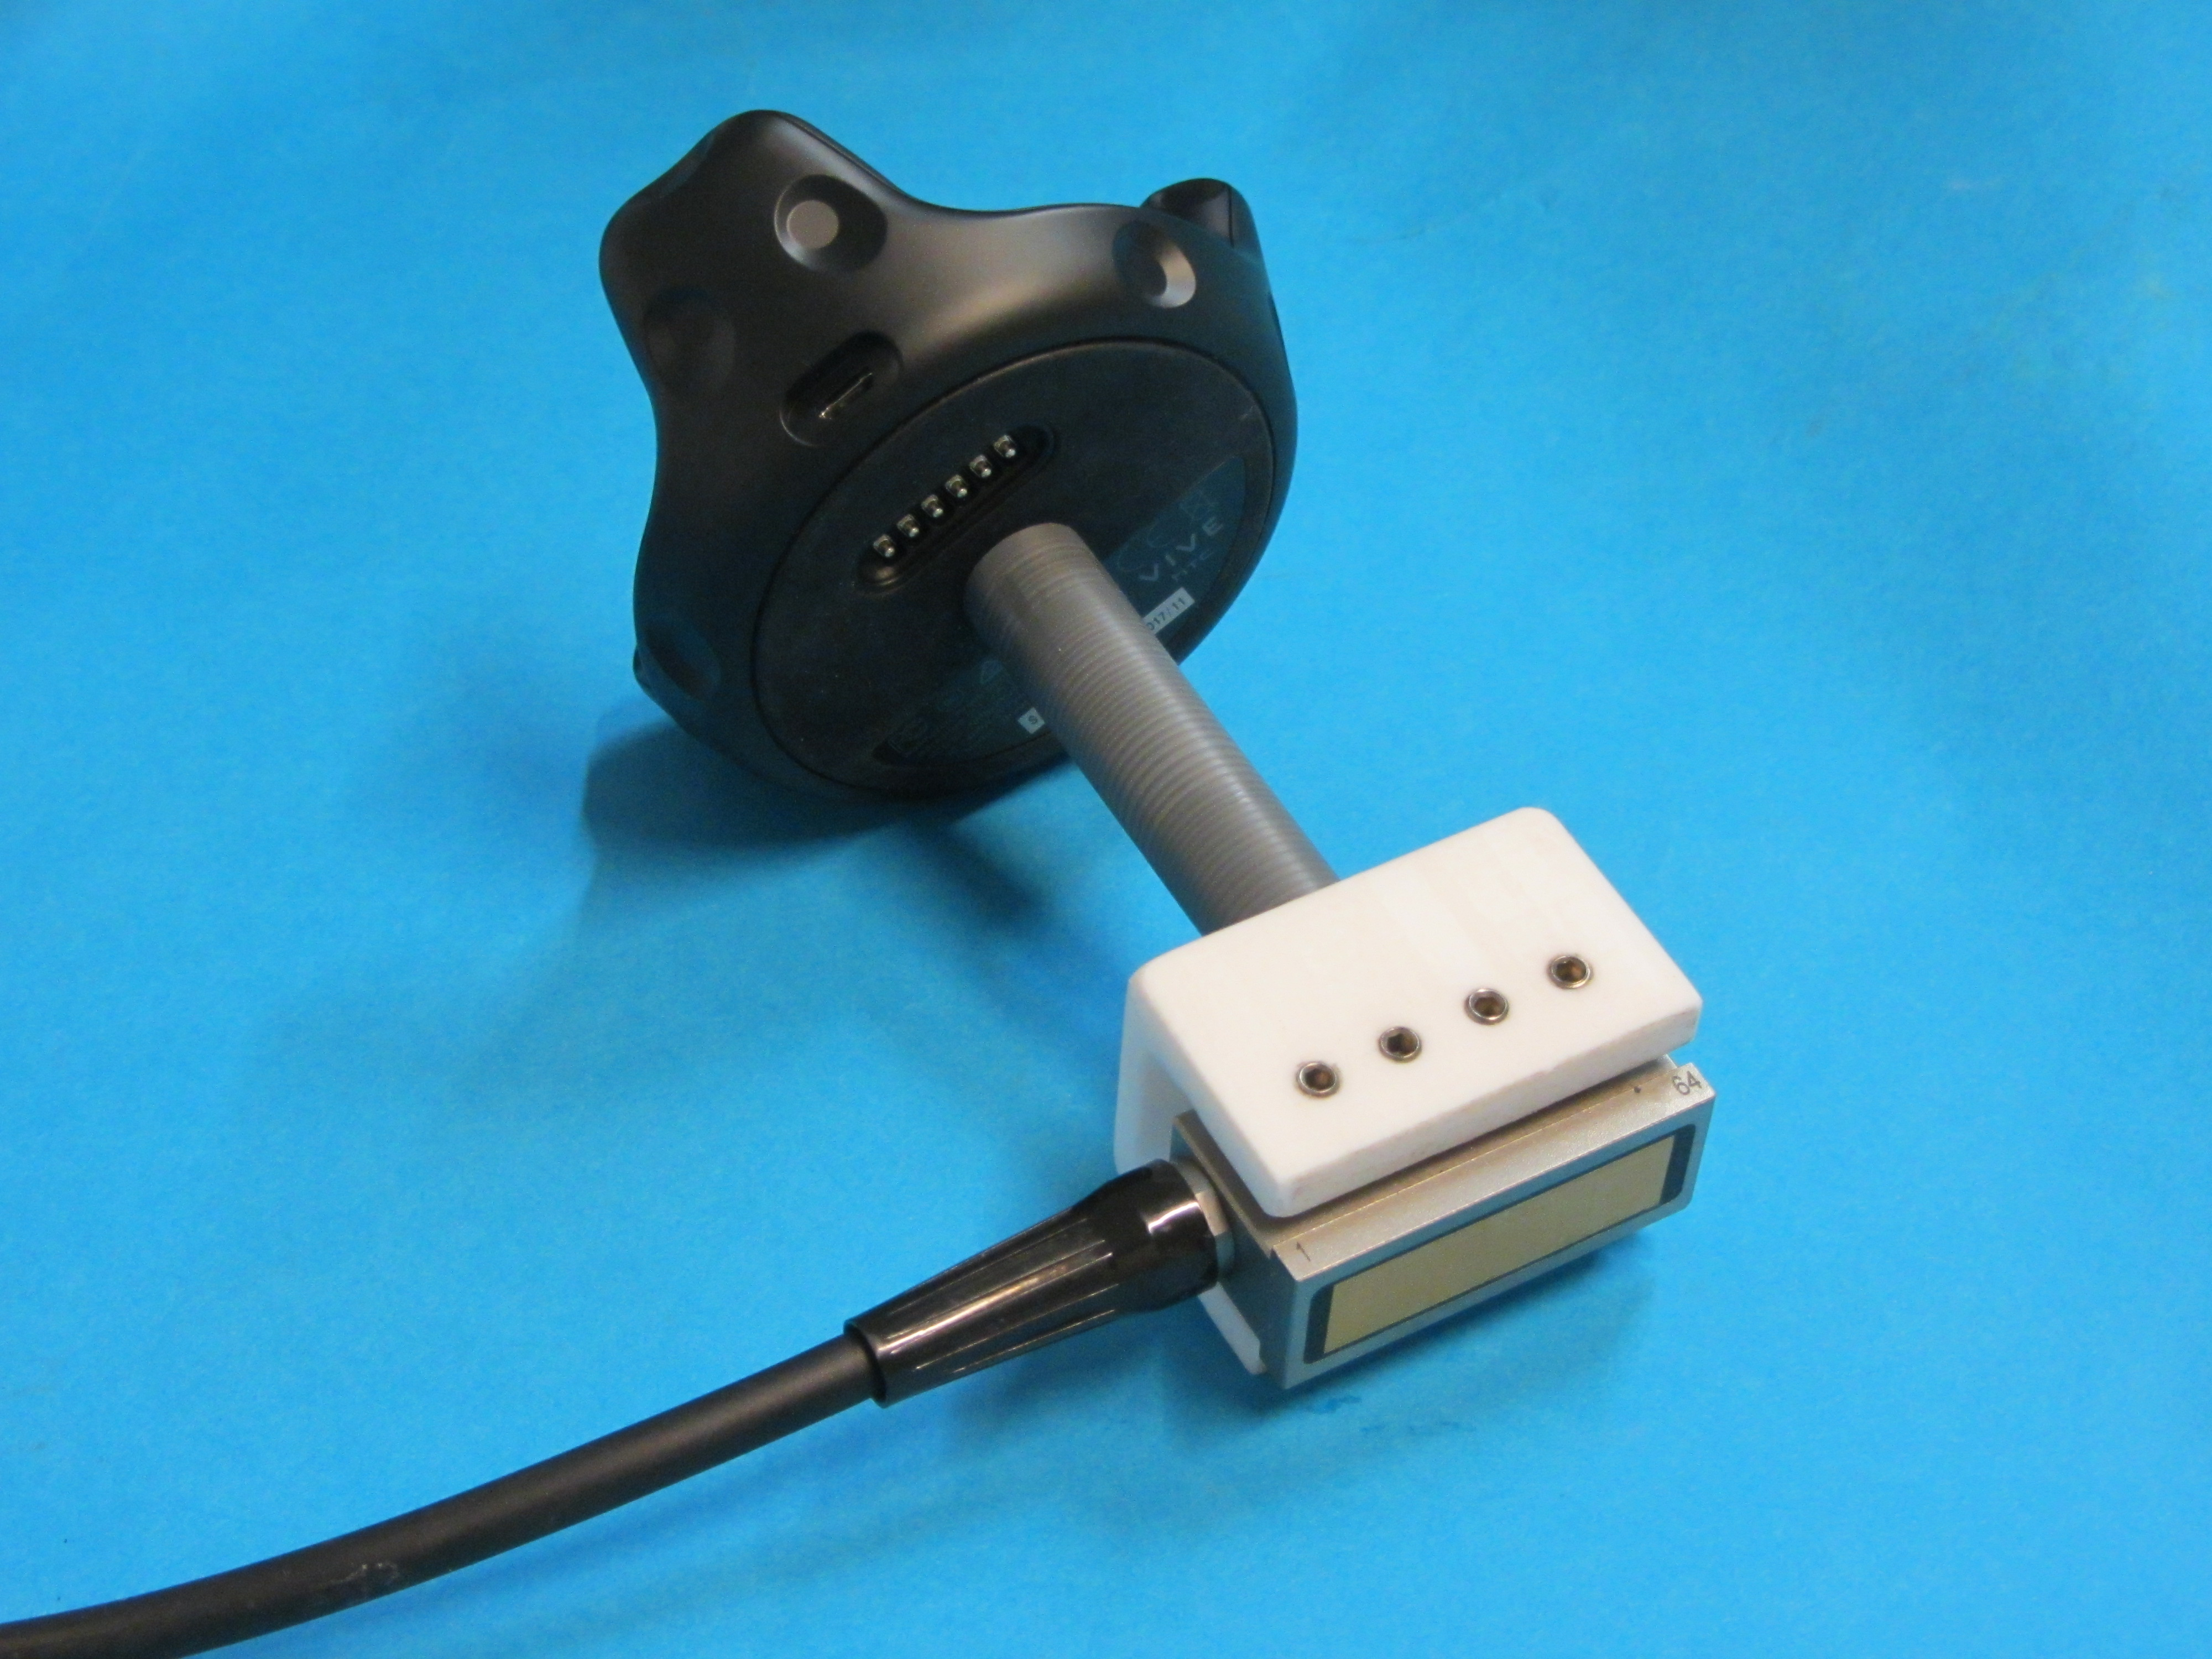
\includegraphics[width=79mm]{images/probemount}
        \caption{\label{fig:probemount} Probemount, that fixes \textit{VIVE-}Tracker to ultrasonic probe.}
    \end{center}
\end{figure}

\subsection{Detection of the coordinate system in worldspace}
The coordinate system of the surface to be measured is detected in two steps:
first a point-cloud of the surface is created by moving the tracked probe across it.
In the next step the parameters of the selected geometry in worldspace are calculated from this point-cloud using the Downhill-Simplex optimization by Nelder and Mead.
In a second step the used coordinate system is picked by placing the tracked probe at the desired origin and pressing the setup button.
As the specimen-geometry is already defined, only one more axis is required to define the orthogonal coordinate system.
this is done by placing the tracked probe on the X-Axis and pressing the setup button.

\subsection{Visualization of the tracking-data}
\label{sec:DrawVsErase}
To visualize the already traced path, a visual feedback is given to the inspector.
The feedback can be implemented in multiple ways, depending on the application.
The path can either be drawn on the surface ({\sc Draw}), erased from a pre-colored area ({\sc Erase}), or be drawn onto a pre-colored area ({\sc Hybrid}) (Figure~\ref{fig:DrawVsErase}).

\begin{figure}[h!]
    \begin{center}
        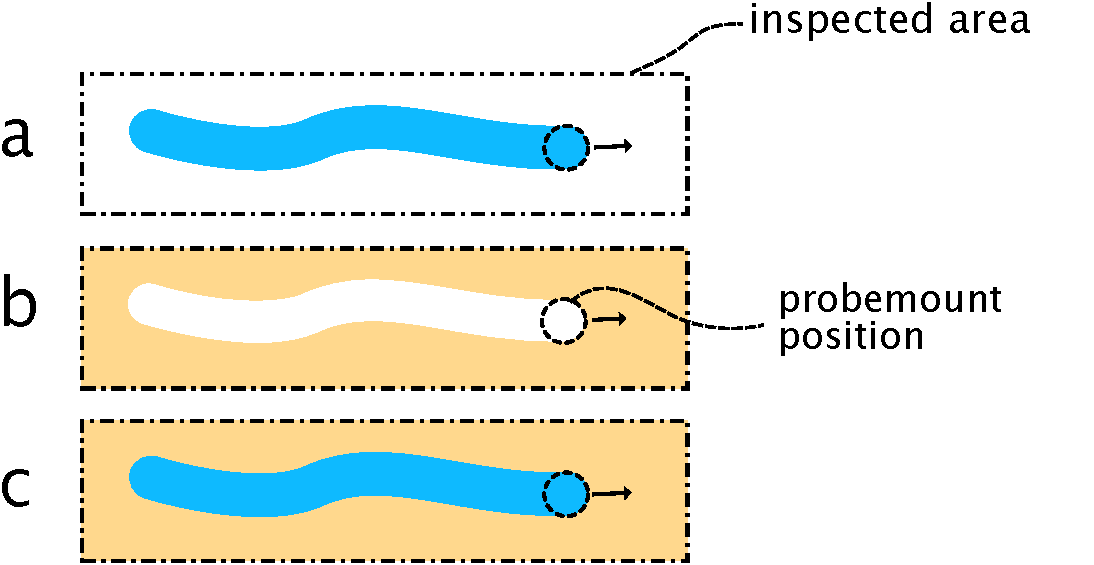
\includegraphics[width=79mm]{images/DrawVsErase}
        \caption{\label{fig:DrawVsErase} Different methods to mark covered area. (a) {\sc Draw} (b) {\sc Erase} (c) {\sc Hybrid}}
    \end{center}
\end{figure}

The main purpose of this visualization is to show possible gaps in the inspection, or to follow a predefined inspection-path.
In the case of SZMF, there is usually no specific inspection-plan that can give a pattern to erase, therefore {\sc DRAW} was implemented.
The AR-view of the application can be seen in Figure~\ref{fig:ARView}.

\begin{figure}[h!]
    \begin{center}
        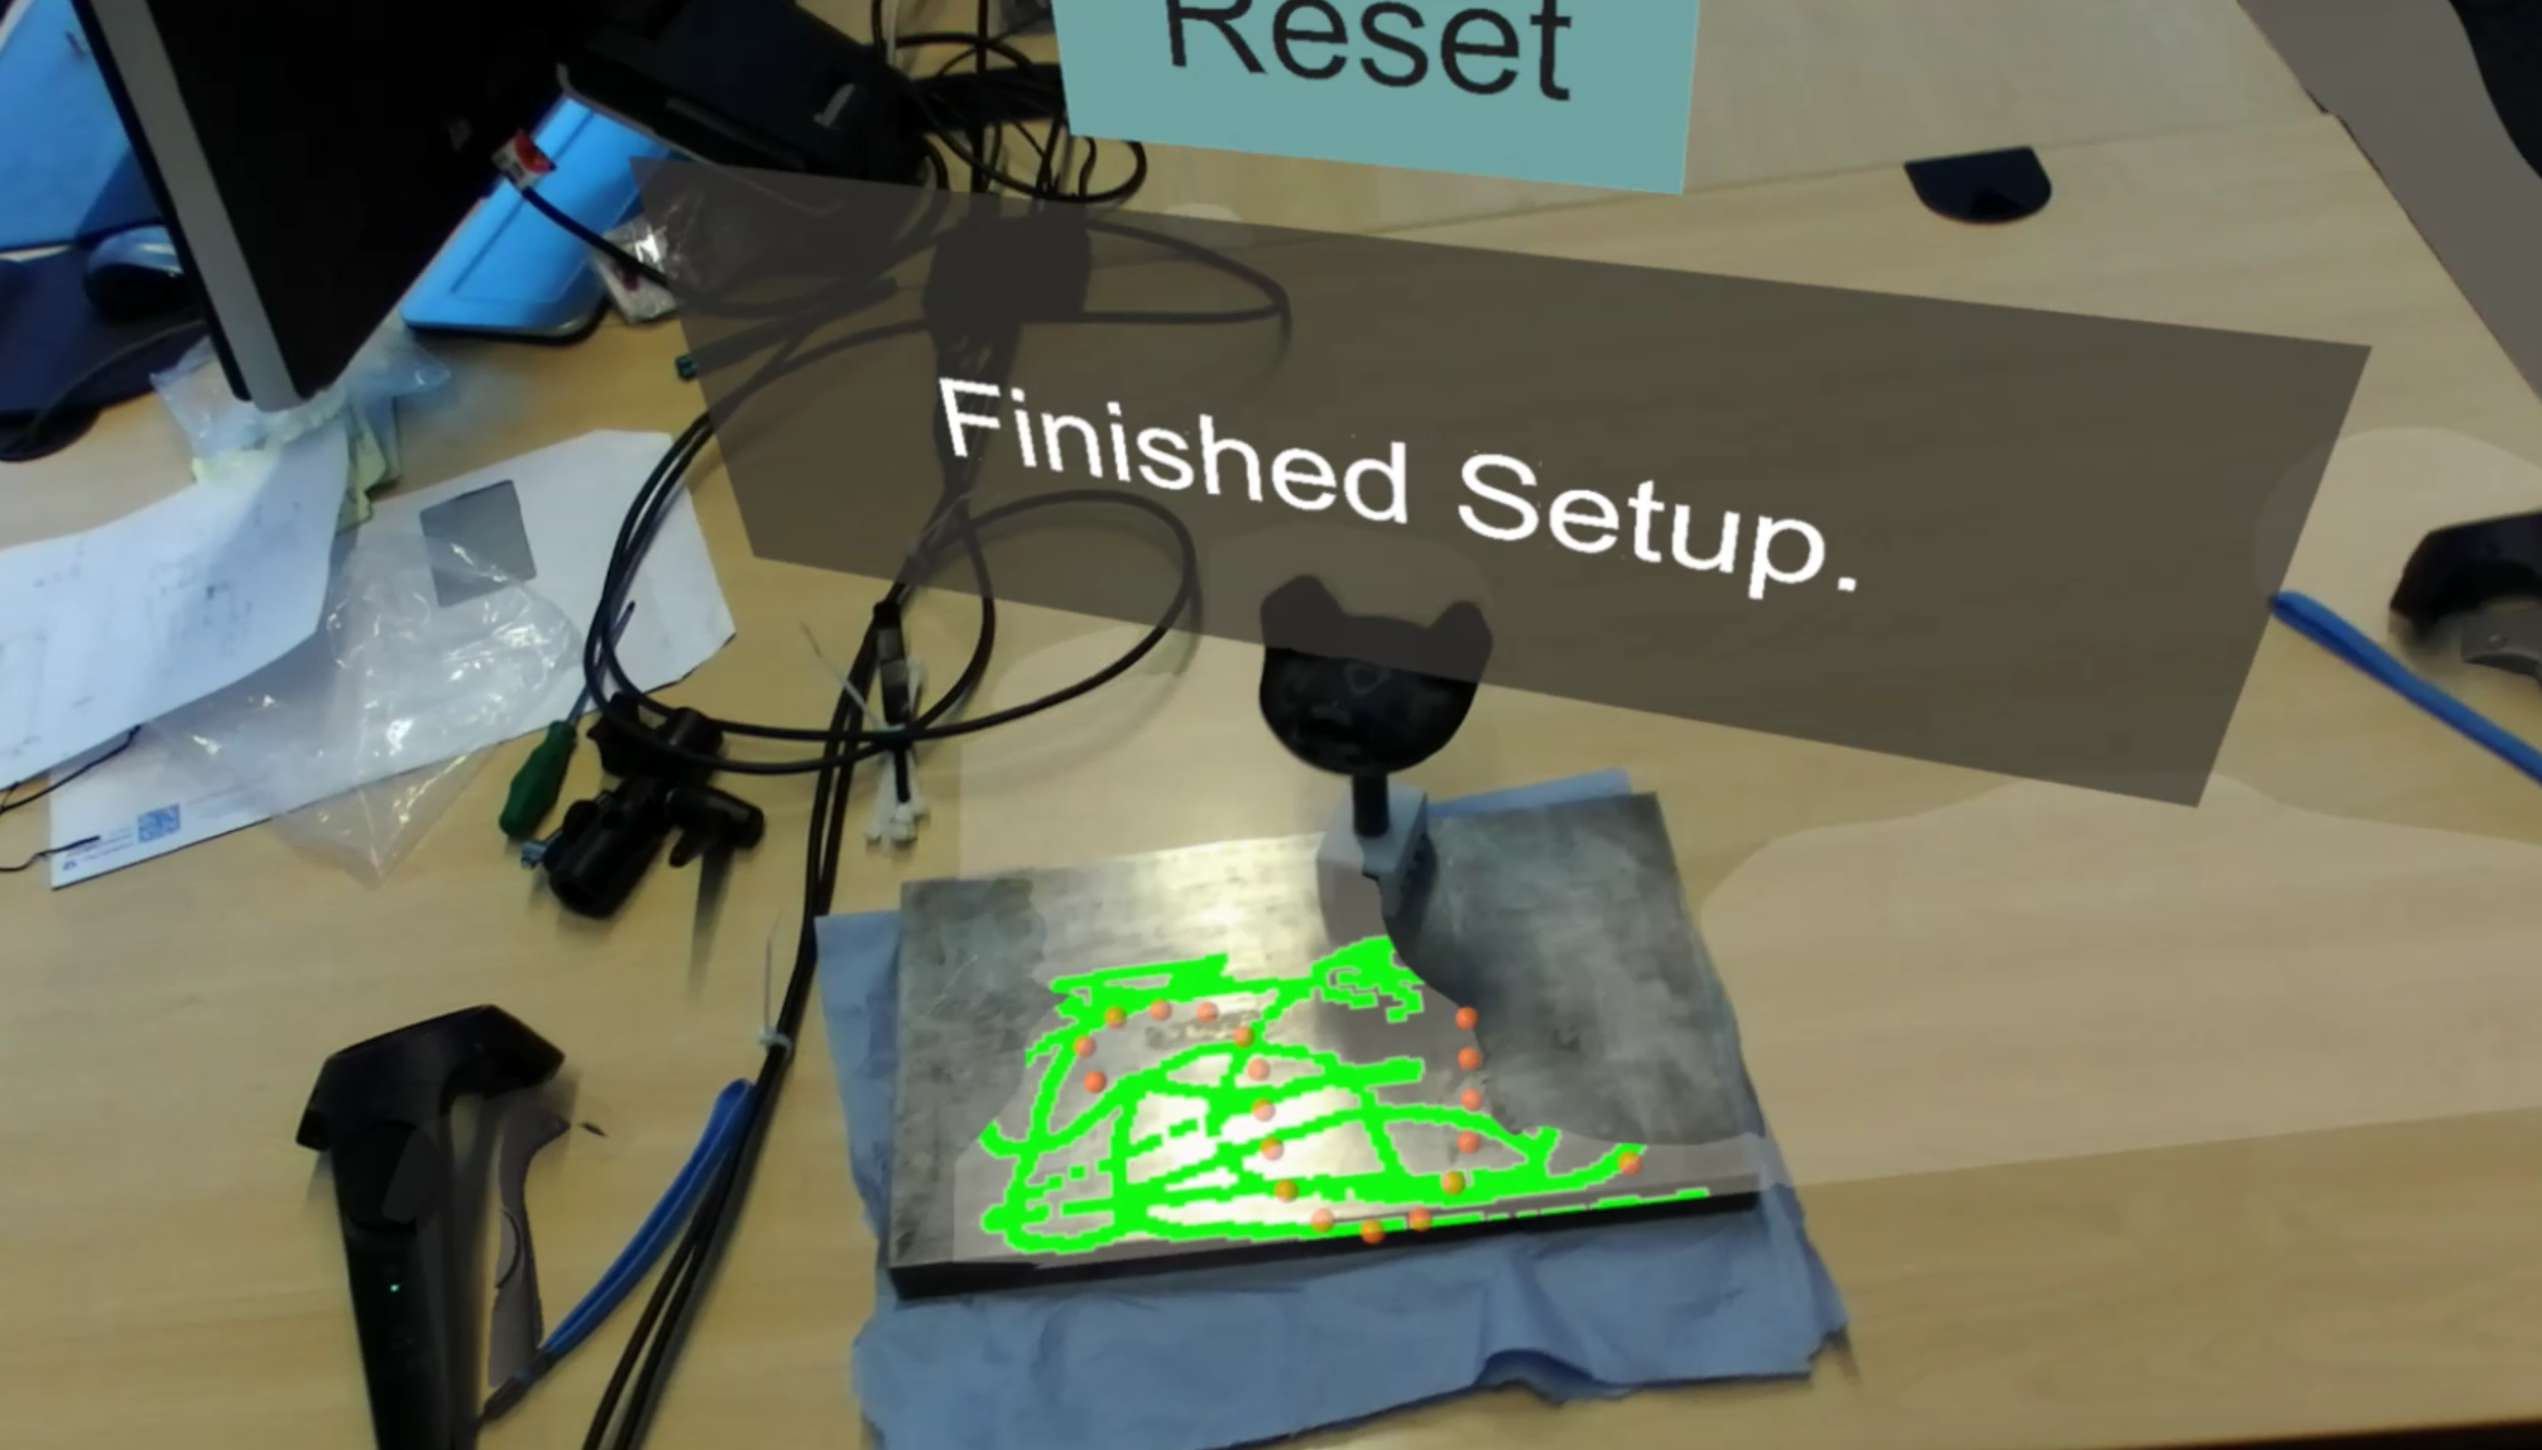
\includegraphics[width=90mm]{images/AR-Screenshot}
        \caption{\label{fig:ARView} AR-view of the application with green drawn path, the probe has covered.}
    \end{center}
\end{figure}

The patches in the surface, where no color can be seen, can be explained by a lack in accuracy of the depth image, generated by the used stereocamera.

\subsection{Continuous and singular logging of position}
The application allows the continuous logging of the probes position.
This protocol can be useful for documenting exactly which path was taken, and where exactly the imperfections were detected.
In addition to that, it is possible to log singular spots and store them for later use.

\section{Evaluation of the \textit{VIVE}-tracker accuracy}
The accuracy of the \textit{VIVE}-Tracker was determined in a experiment using an automated X-Y-scanner.
Both \textit{VIVE}-Basestations were positioned on opposite corners of the scanner, though one at a greater distance (figure~\ref{fig:precisionMeasurementSetup}).

\begin{figure}[h!]
    \begin{center}
        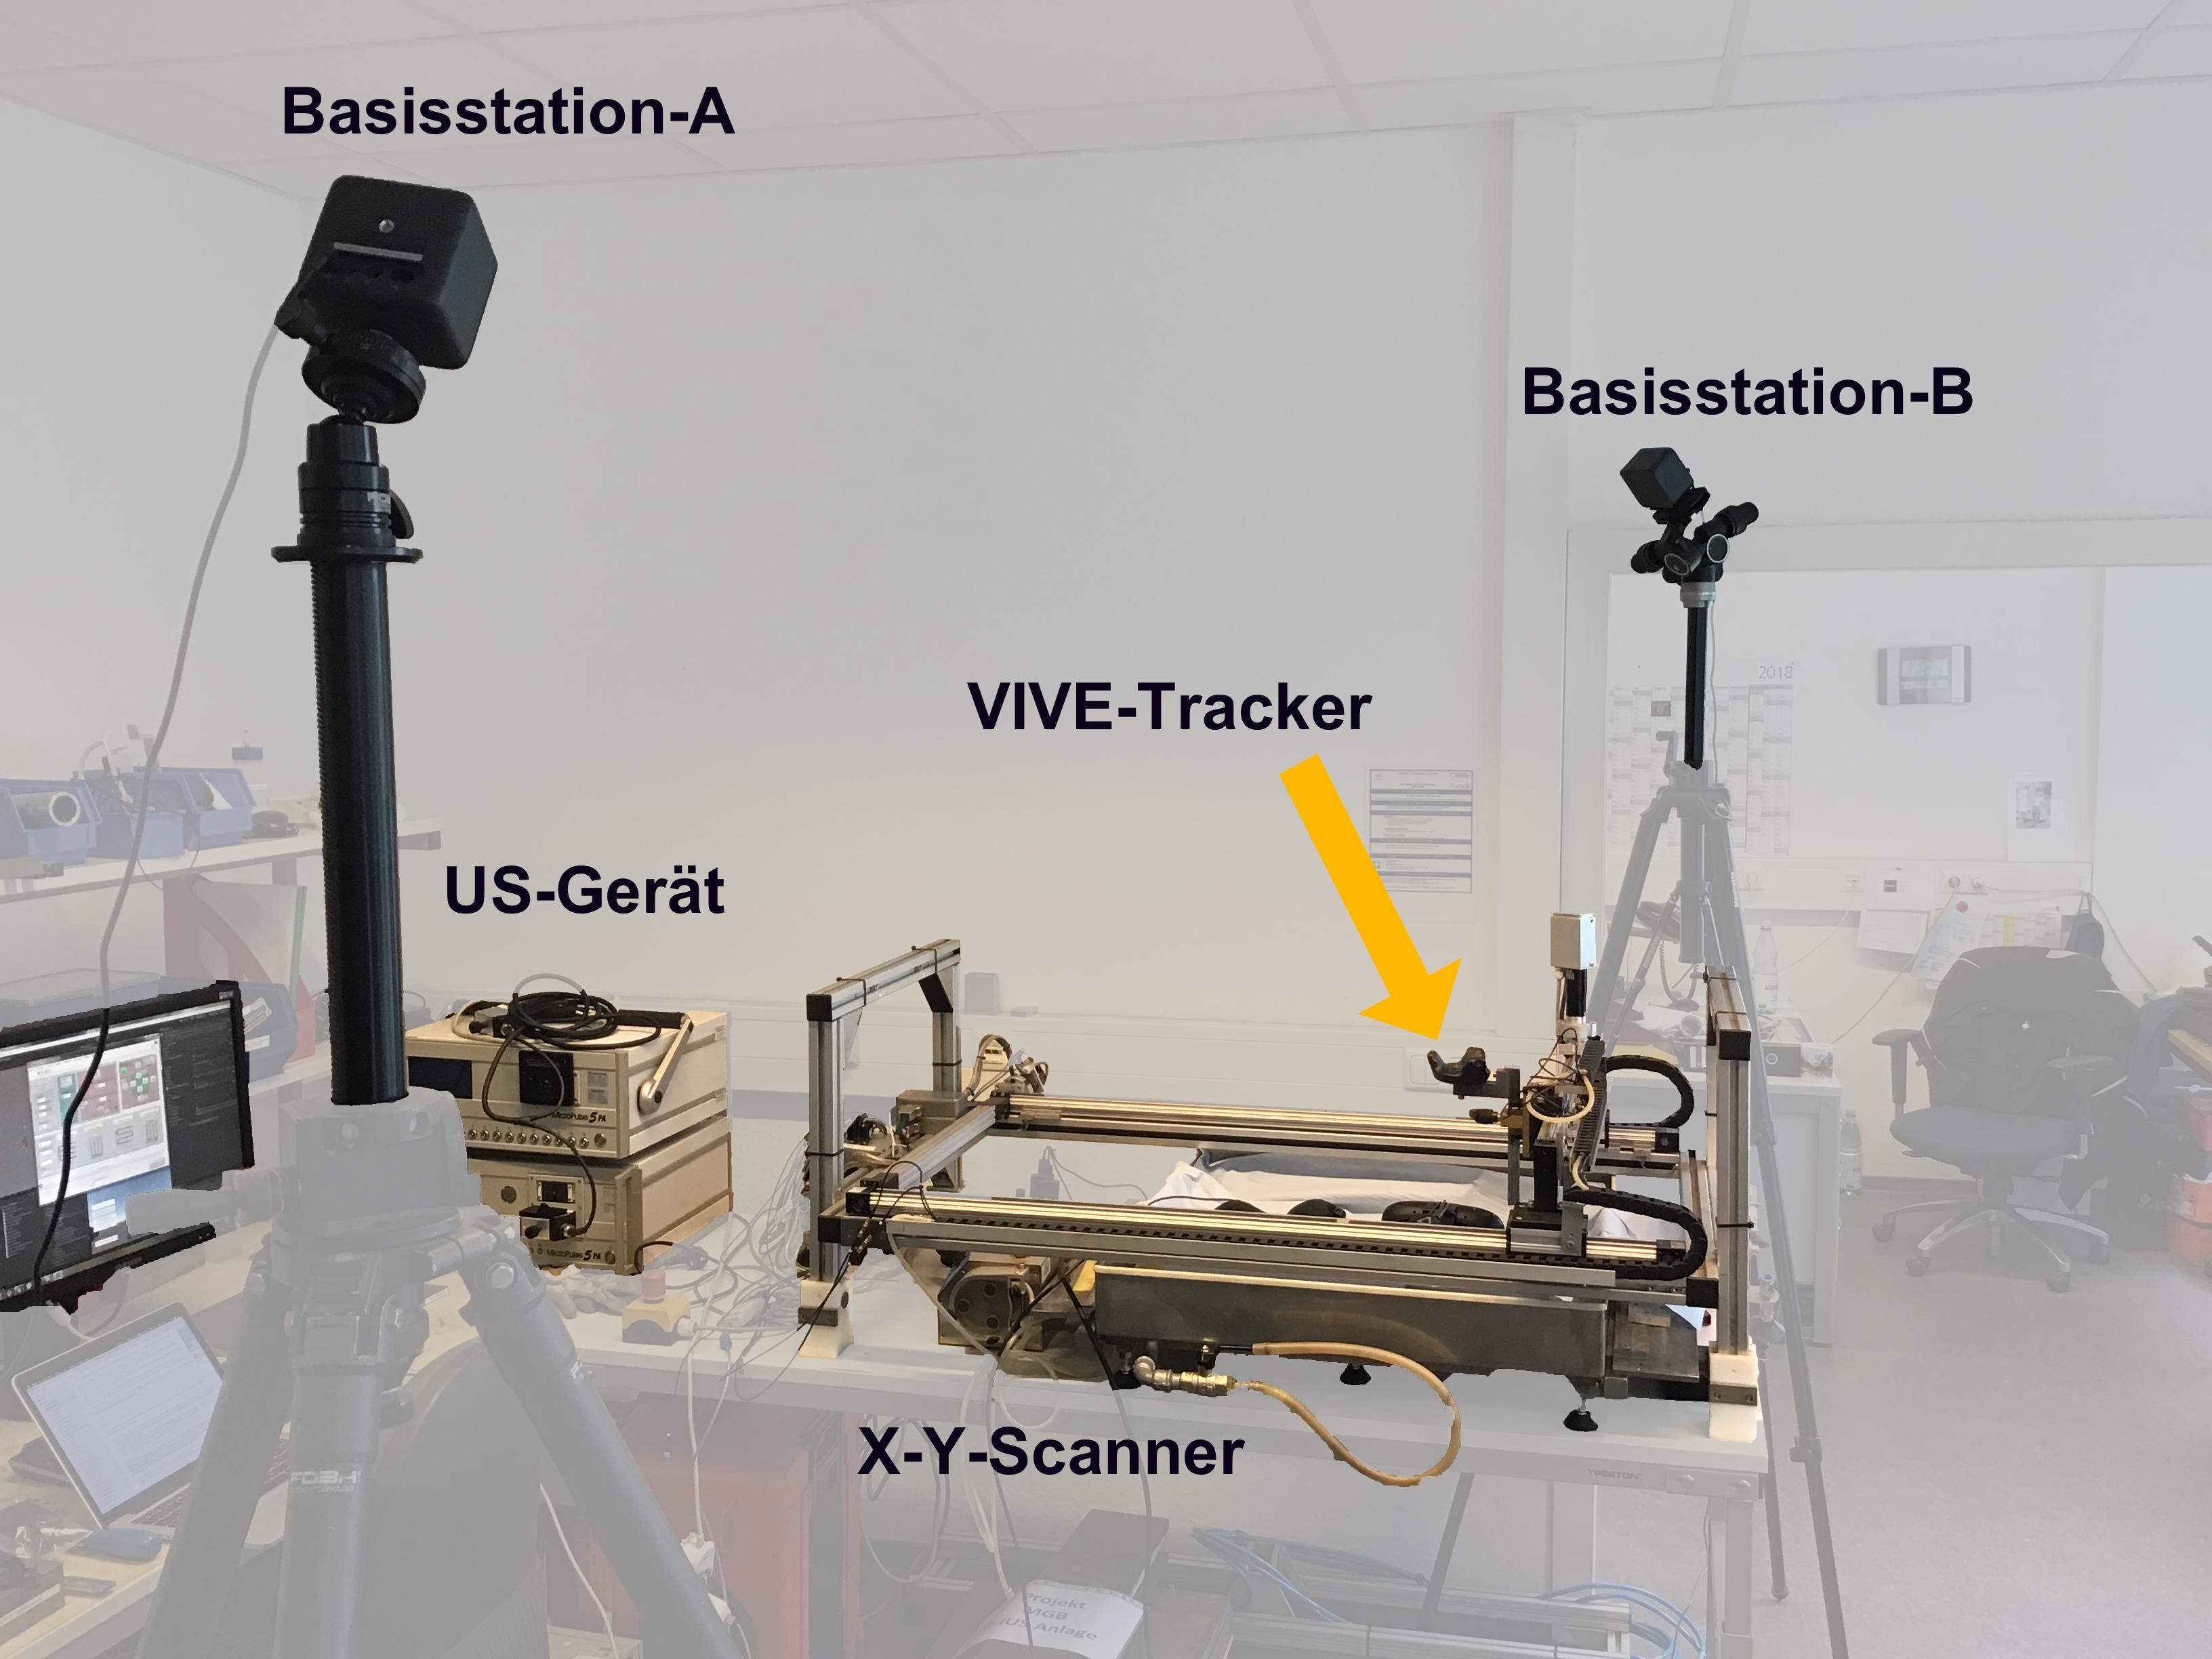
\includegraphics[width=120mm]{images/PrecisionMeasurement}
        \caption{\label{fig:precisionMeasurementSetup} Setup for the evaluation of the \textit{VIVE}-Precision.}
    \end{center}
\end{figure}

The results show a decline in quality as the surveypoints get closer to the closer basestation (basestation-B in figure~\ref{fig:precisionMeasurementSetup}) with an error up to 18\,mm.
In the opposite corner the values had a quality of about 1-2\,mm.
This can be explained by the rapidly declining quality as the proximity to the basestation is too small.

\section{Conclusion}

\begin{figure}[h!]
    \begin{center}
        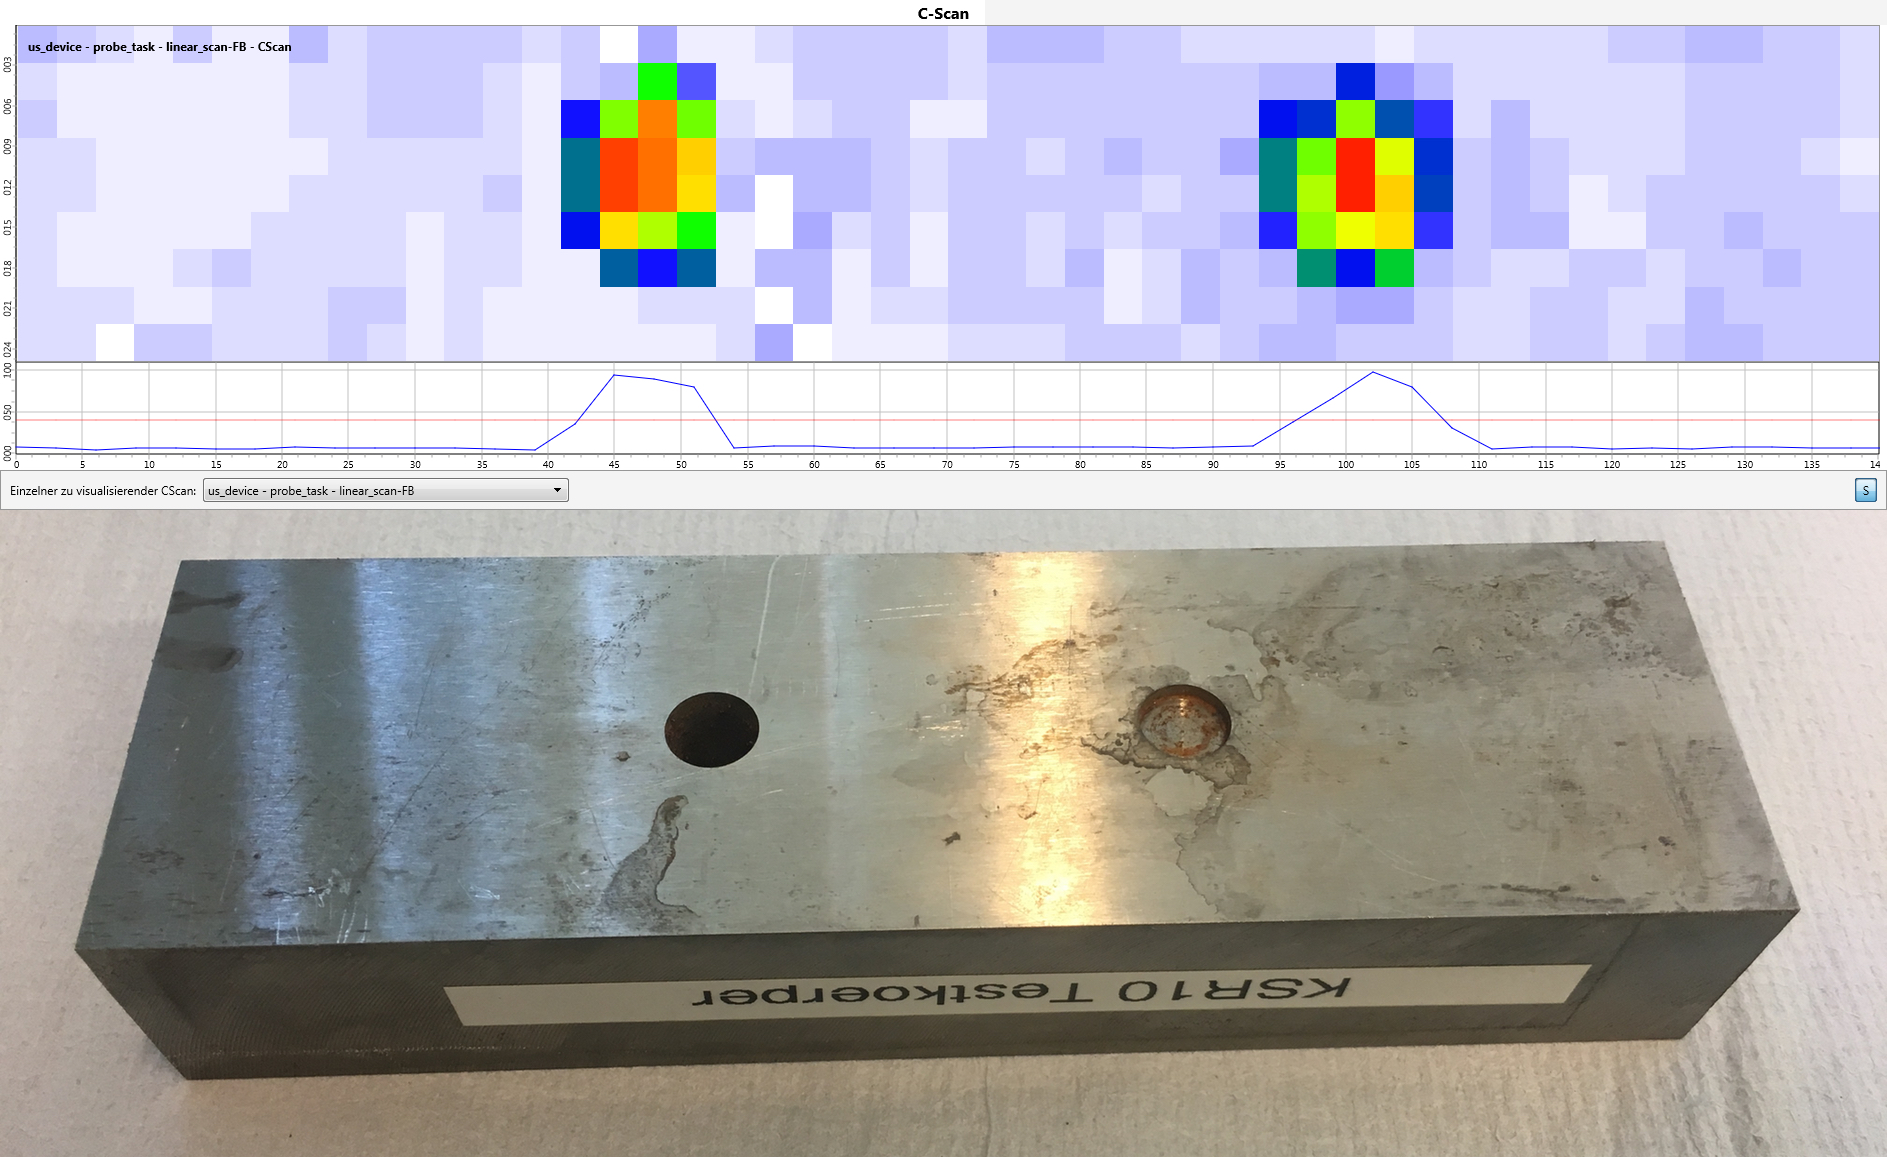
\includegraphics[width=100mm]{images/CScanARUS}
        \caption{\label{fig:resultCScan} C-Scan generated with the \textit{VIVE}-tracking system}
    \end{center}
\end{figure}

\VRARsetbibstyle
\bibliography{bibliography}

\end{document}
